\subsection{Section 4.2.2-Style Effectiveness Evaluation}

The following figures reproduce the effectiveness-evaluation style of Section 4.2.2 using the ArduPilot SITL dataset and the final V9/p99\_abs/W10\_N3\_mean1x recovery configuration.

\begin{figure*}[t]
    \centering
    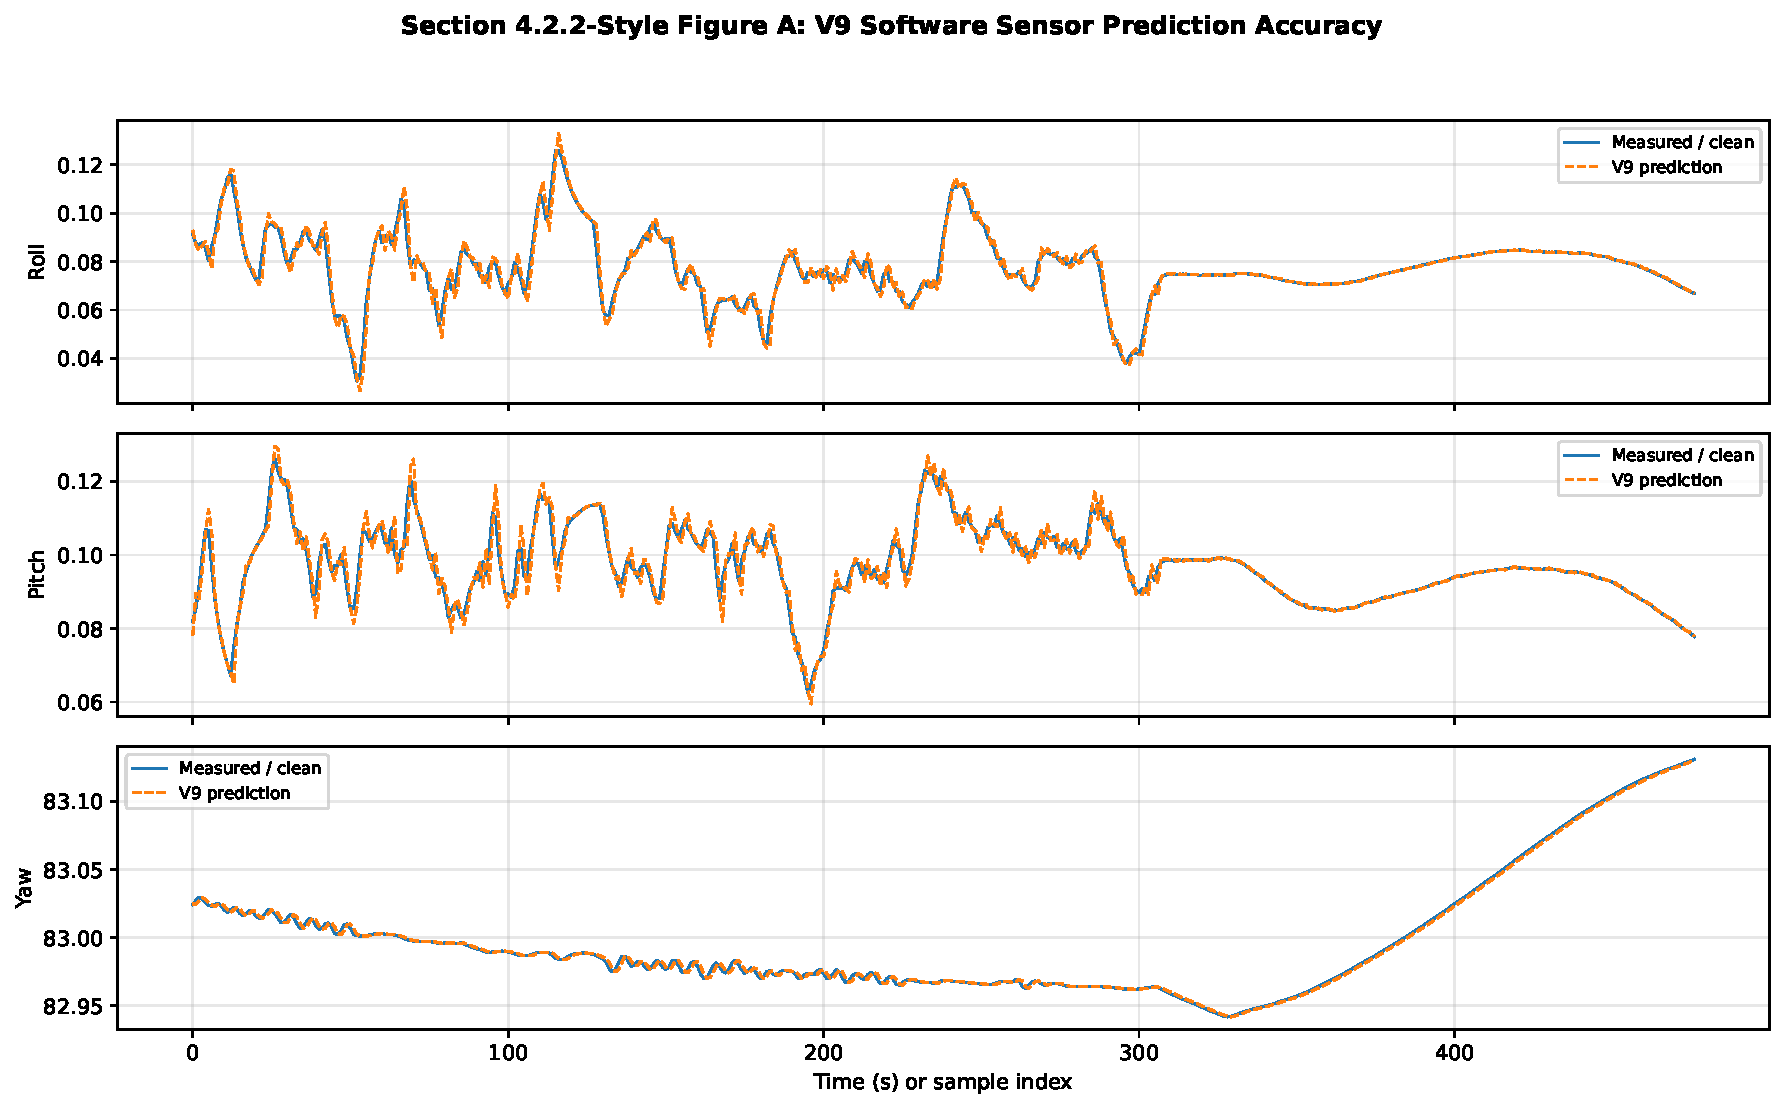
\includegraphics[width=0.95\textwidth]{phase7_section_4_2_2_effectiveness_figures/figure_4_2_2_a_v9_prediction_accuracy_v2.pdf}
    \caption{V9 software-sensor prediction accuracy. The V9 trained hybrid predictor estimates the future attitude state using information available at time $k$ and closely follows the measured clean Roll, Pitch, and Yaw signals.}
    \label{fig:v9_prediction_accuracy_v2}
\end{figure*}

\begin{figure*}[t]
    \centering
    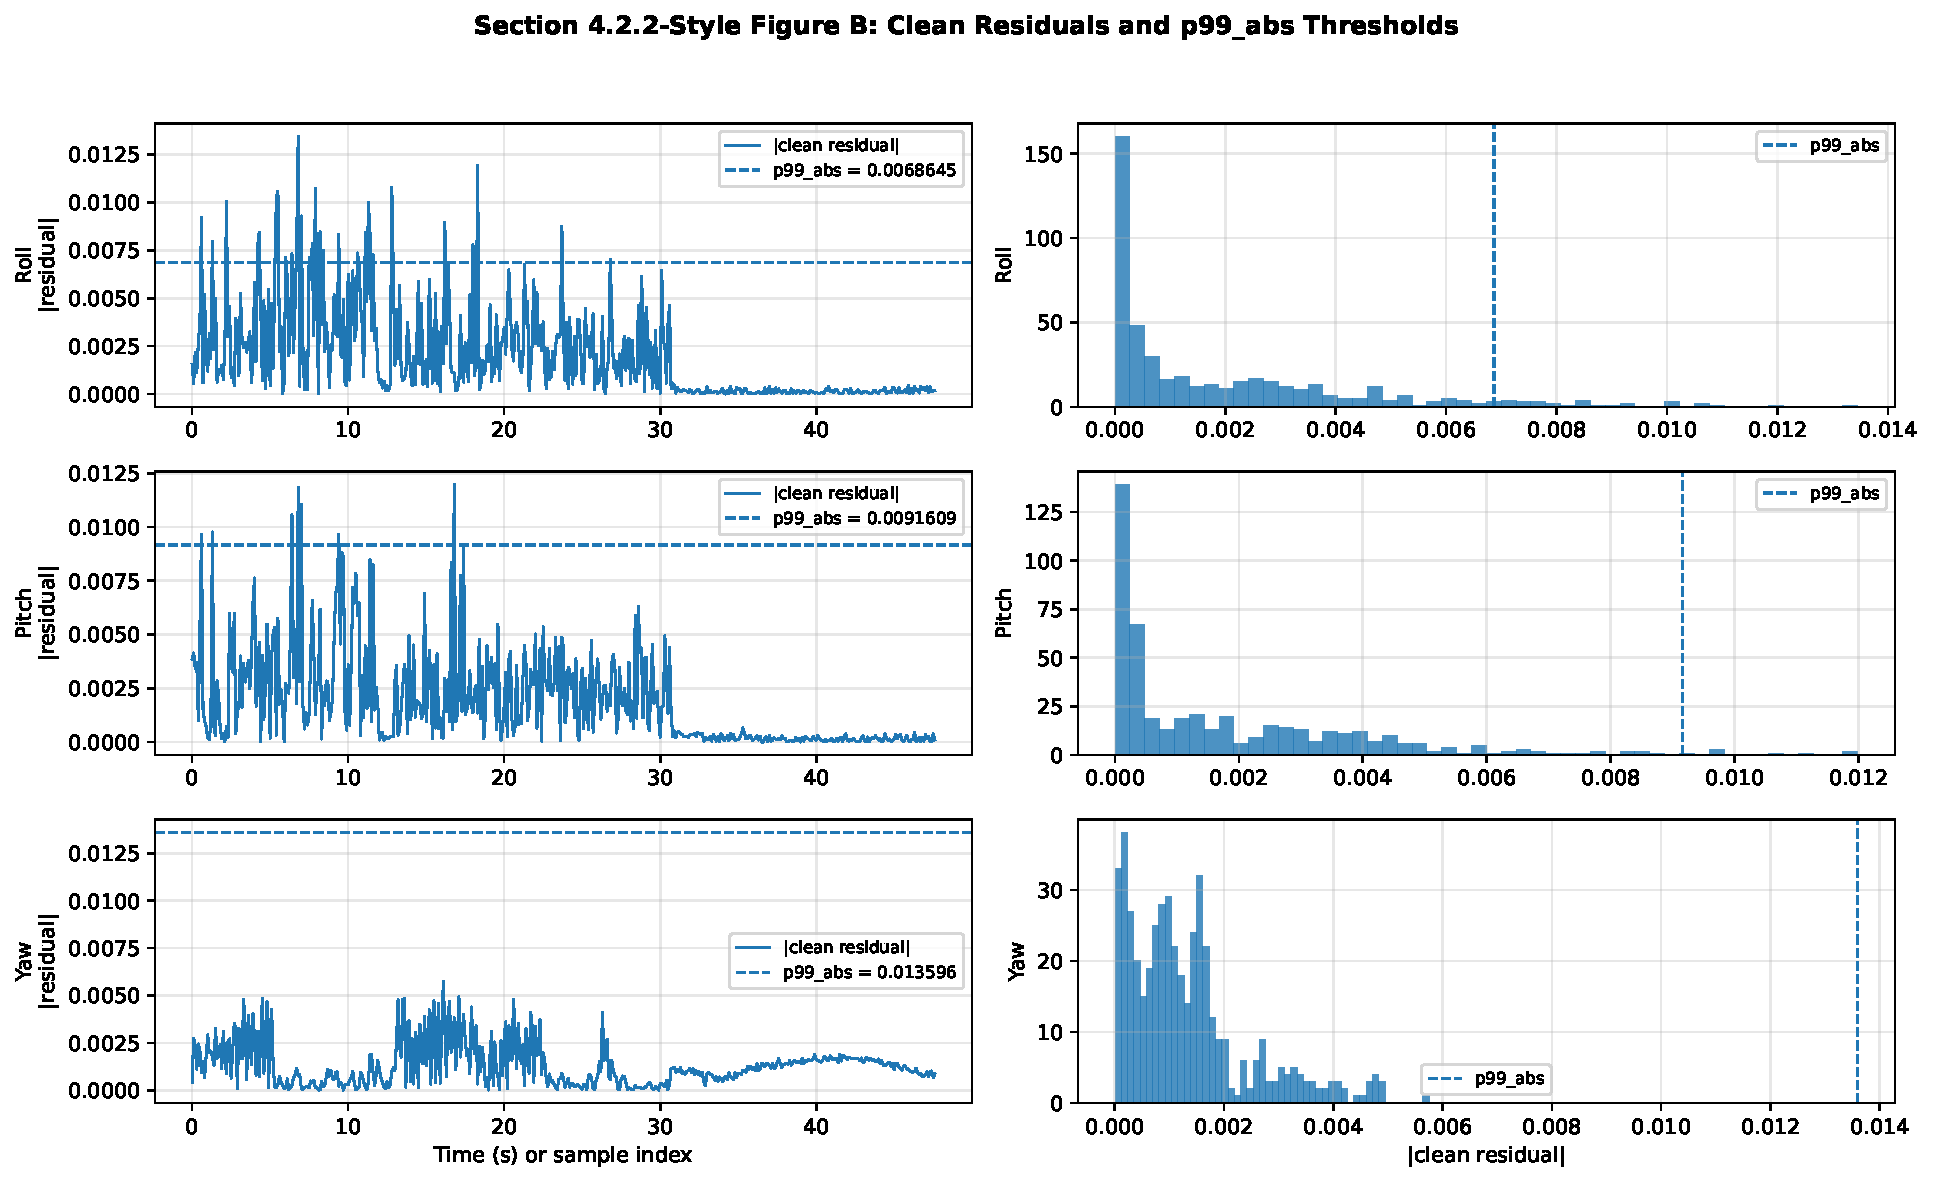
\includegraphics[width=0.95\textwidth]{phase7_section_4_2_2_effectiveness_figures/figure_4_2_2_b_clean_residual_threshold_v2.pdf}
    \caption{Clean residual behavior and $p99\_abs$ thresholds. The thresholds are computed from clean residual distributions and are used as the abnormal-deviation boundary during attack detection.}
    \label{fig:clean_residual_threshold_v2}
\end{figure*}

\begin{figure*}[t]
    \centering
    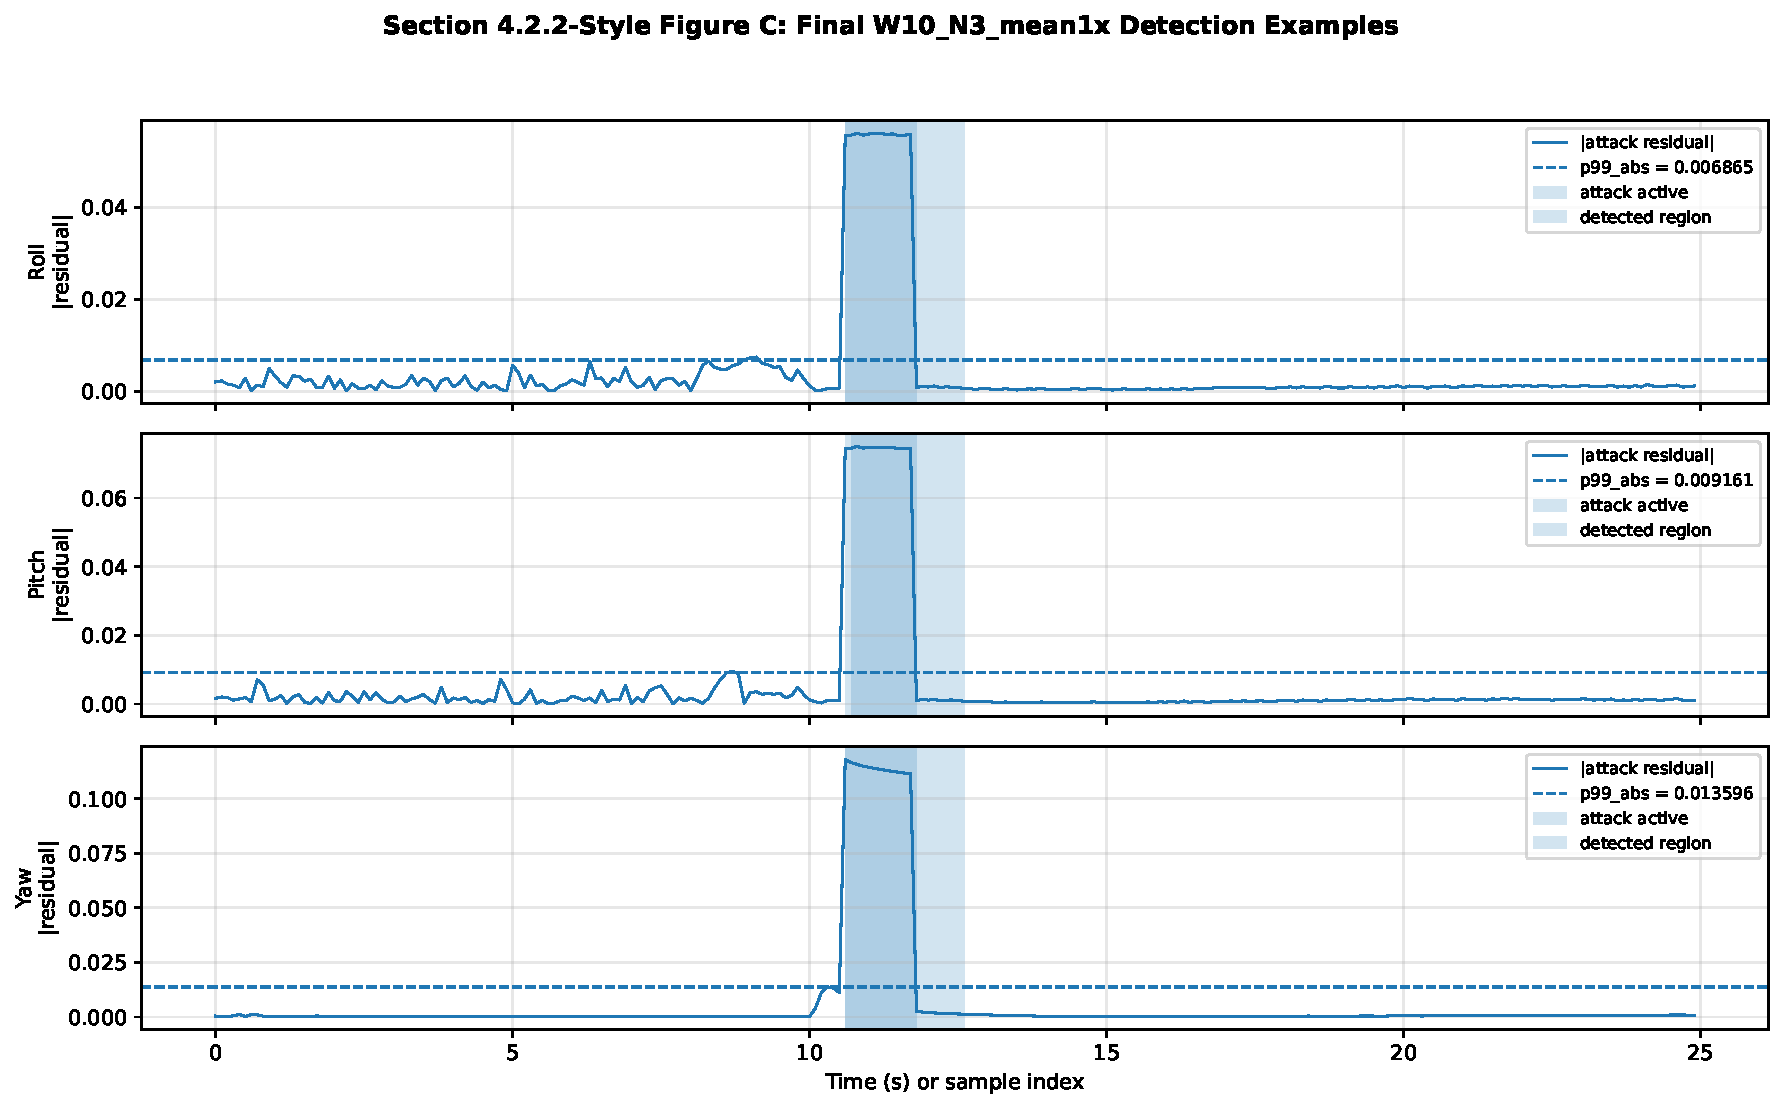
\includegraphics[width=0.95\textwidth]{phase7_section_4_2_2_effectiveness_figures/figure_4_2_2_c_W10_N3_detection_examples_v2.pdf}
    \caption{Final W10\_N3\_mean1x window-detection examples. The detector declares an attack when at least three residual threshold violations occur inside a ten-sample window.}
    \label{fig:w10n3_detection_examples_v2}
\end{figure*}

\begin{figure*}[t]
    \centering
    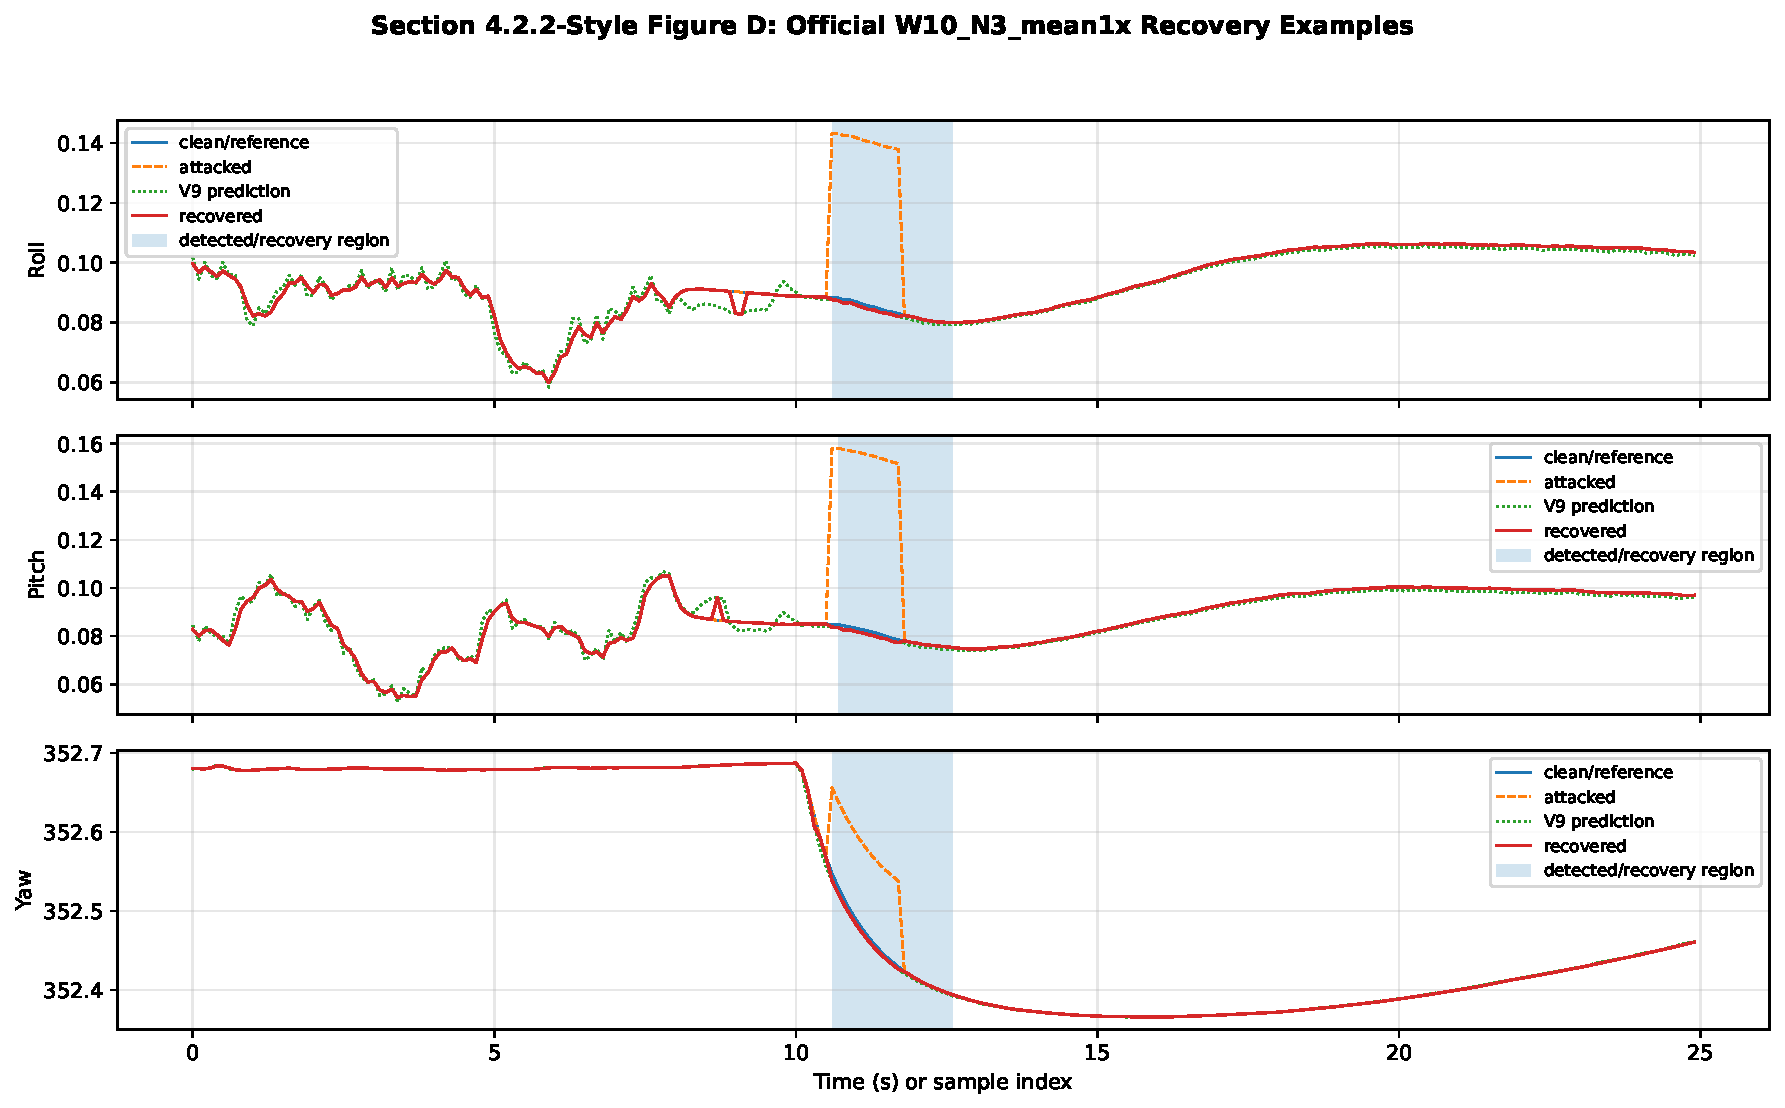
\includegraphics[width=0.95\textwidth]{phase7_section_4_2_2_effectiveness_figures/figure_4_2_2_d_W10_N3_recovery_examples_v2.pdf}
    \caption{Official W10\_N3\_mean1x recovery examples. During detected attack periods, the corrupted measurement is replaced by the V9 software-sensor prediction.}
    \label{fig:w10n3_recovery_examples_v2}
\end{figure*}

\begin{figure}[t]
    \centering
    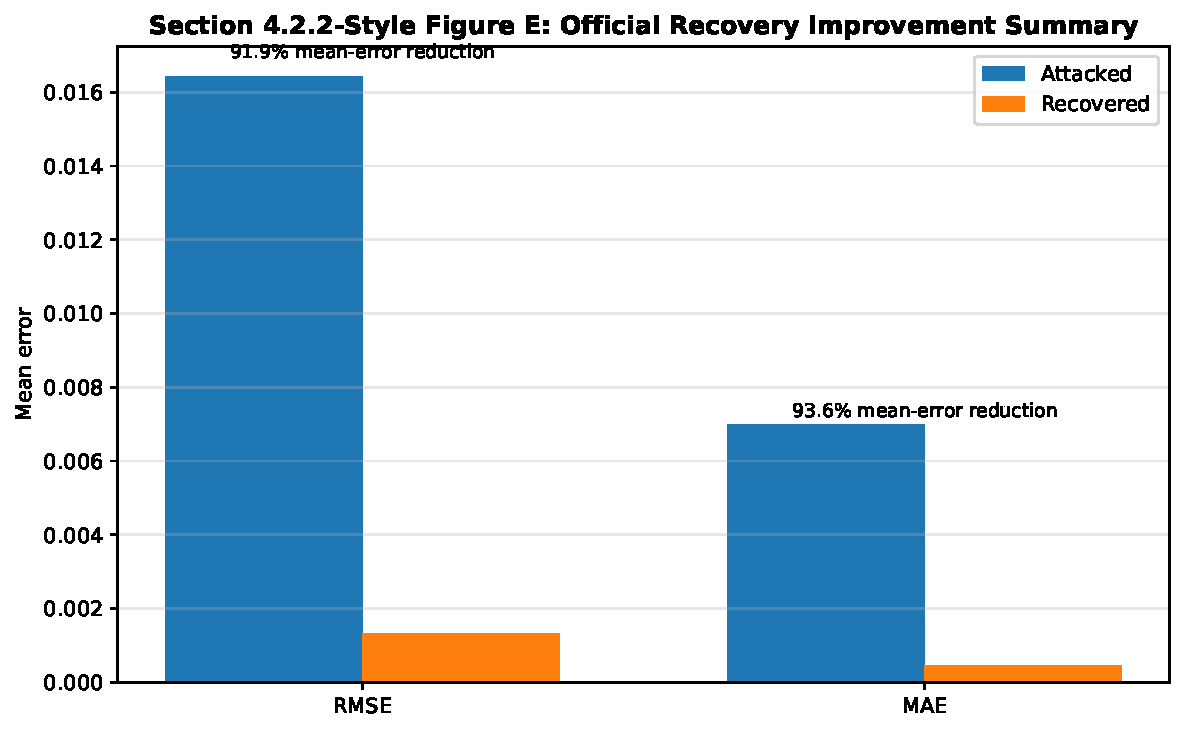
\includegraphics[width=0.48\textwidth]{phase7_section_4_2_2_effectiveness_figures/figure_4_2_2_e_recovery_improvement_summary_v2.pdf}
    \caption{Official recovery improvement summary. The recovered signal substantially reduces mean RMSE and MAE compared with the attacked signal.}
    \label{fig:recovery_improvement_summary_v2}
\end{figure}
